\section{Specifications}
\newcounter{rulei}[subsection]
\newcommand{\rcnii}{\stepcounter{rulei}\arabic{section}.\arabic{subsection}.\arabic{rulei}}
\renewcommand{\labelenumi}{\rcnii}

\subsection{Arena}
\begin{enumerate}
\item The match arena floor is an 8m x 8m square.  The tolerance of the two arena dimensions is $\pm0.25m$.
\item The floor of the arena is made of white plastic coated hardboard.  White Gaffer tape will be in place over the joints between hardboard sheets.
\item The arena walls are $600\pm30mm$ high and are made of the same material as the arena floor.
\item The arena is encased in a scaffolding structure, which $2.6m \pm0.1m$ tall.  The scaffolding structure is covered in netting in order to prevent balls from escaping from the arena.
\end{enumerate}

\subsection{Balls}
\label{balls}
\begin {enumerate} 
\item Balls have a radius of 55mm, and can be purchased from Argos with the part number 366/5514.  Each team's kit contains a small number of these.
\item The following ball colours will be used: red, blue, yellow and green.
\end {enumerate}

\subsection{Zones}
\begin {enumerate}
\item The arena contains 4 zones.  Each zone occupies one quarter of the arena and has an associated colour and net.  Figure~\ref{fig:arena} shows the dimensions and colours of the zones.
\item The zone is bounded by a border of black Gaffer tape stuck to the arena floor.  Each arm of the Gaffer tape cross has a different width.  The four widths are 50, 75, 100 and 125mm.
\end {enumerate}

\begin{figure}
\begin{center}
\includegraphics[keepaspectratio, width=\textwidth]{./images/arenadim.pdf}
\caption{\label{fig:arena}Arena dimensions and markings.}
\end{center}
\end{figure}

\begin{figure}
\begin{center}
\includegraphics[keepaspectratio, scale =1]{./images/colours.pdf}
\caption{\label{fig:zone}Zone and net colours.}
\end{center}
\end{figure}

\subsection{Nets}
\begin{enumerate}
\item The arena contains 4 nets.  Each net is a horizontal triangle of netting, held up by a diagonal rod of scaffold. Figure~\ref{fig:nets} shows the dimensions and positioning of the nets.
\item Square sections of the arena wall are coloured at their intersection below the nets, as shown in figure~\ref{fig:nets}.
\end{enumerate}

\begin{figure}
\begin{center}
\includegraphics[keepaspectratio, scale =1]{./images/net.pdf}
\caption{\label{fig:nets}Isometric view of the arena corner.}
\end{center}
\end{figure}

\subsection{Robot Flags}
\label{sec:flags}
All robots must have a flagpole so that two flags can be mounted upon it:
\begin{description}
\item[Team Flag] The team flag is to be designed and created by the team.  It is optional and recommended.  The team flag allows the robot to be easily identified.  This flag must be mounted between 700mm and 900mm off the ground.  It must not extend more than 200mm from the flagpole.

The team flag must not sag below 700mm above the ground.
\item[Match Flag] The match flag is to be supplied by Student Robotics at the start of every match.  The match flag will slot over the top 100mm of the flagpole.  The top 100mm of the flagpole must have an external diameter of $5\pm1$mm so that the match flag can slot over it.  The match flags have an end-cap so that they will not slide down the flagpole.
\end{description}

The flagpole must be removable so that the robot can be placed within a box to check the size limit.  A diagram of the flagpole arrangement can be found in figure~\ref{fig:flag}.

\begin{figure}
\begin{center}
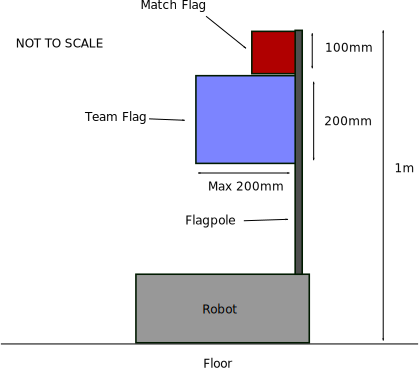
\includegraphics[keepaspectratio, scale =1]{./images/flag.png}
\caption{\label{fig:flag}Flagpole Dimensions}
\end{center}
\end{figure}
\clearpage